
\section{Určenie náklonu zbrane}
\label{sec:urcenienaklonuzbrane}
Druhý z cieľou tejto práce je určenie náklonu zbrane v obraze.
Tento náklon bude určeny v 3 osách.
Dôležité je spomenúť že názvy ós sú pomenované podľa tých ktoré sa používajú v letectve, vid. obrázok \ref{pic:airplaneaxis}.
\begin{figure}[H]
    \centering
    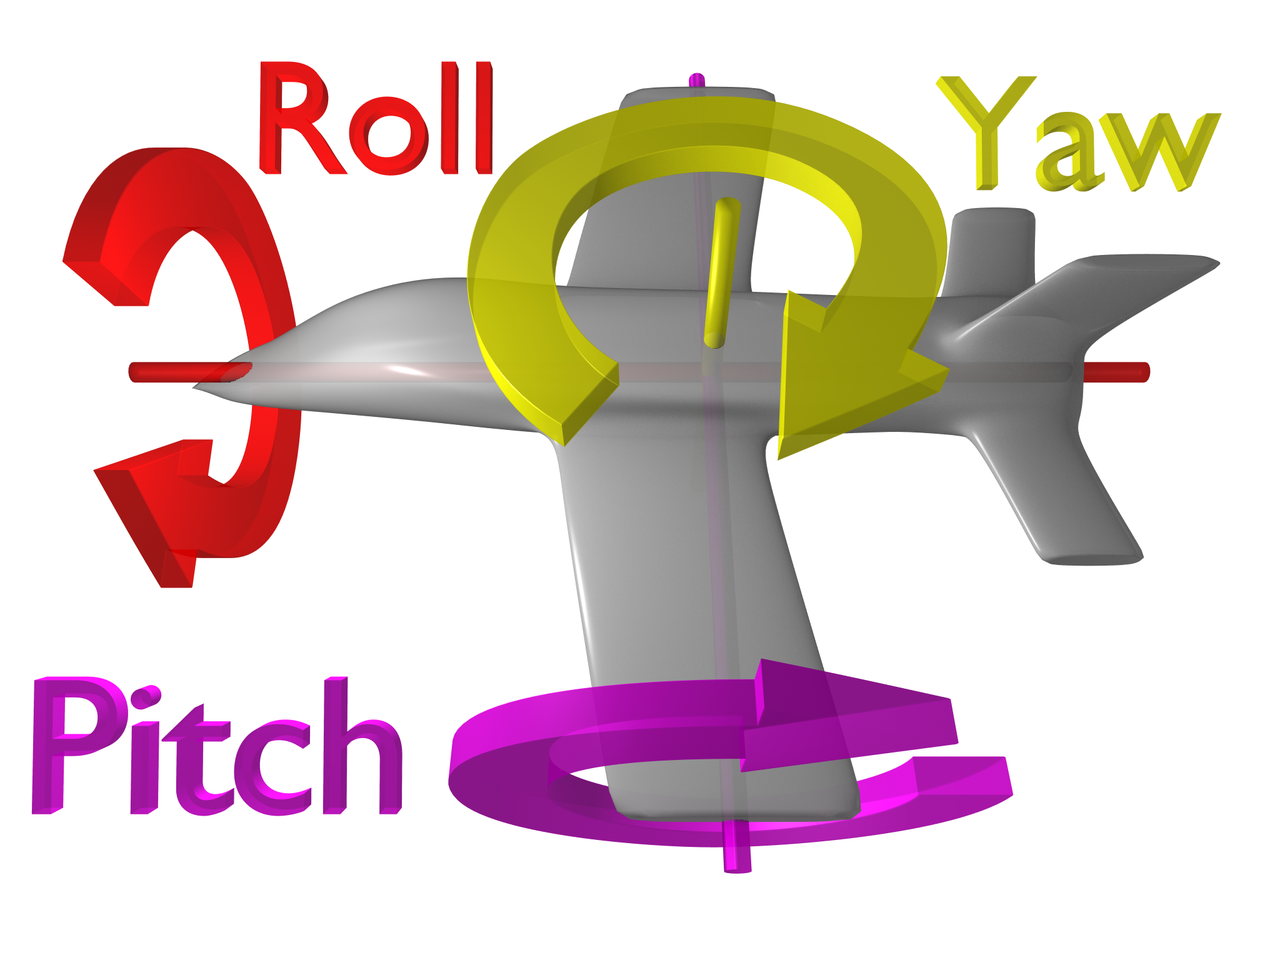
\includegraphics[width=0.5\textwidth]{airplane-axis}
    \caption{Mená ós pre letectvo.}
    \label{pic:airplaneaxis}
\end{figure}

Tento problém je môžné preniesť do klasifikácie, preto pre riešenie tohto problému budú použité konvolučné neurónové siete, ktorých všeobecná architektúra je popísana v \ref{sec:architekuraCNN}.
Výsledok poslednej vrtsvy softmax klasfikátora bude 72 výstupov ktoré budú určovať o aký uhol je zbraň natočená.
Každá zo 72 kategórií bude zastupovať rozpätie 5 stupňov, ciže celkovo sa určí náklon zbrane v celom rozsahu od 0 do 360 stupňov.

Postup predspracovania obrazu bude rovnaký ako pri klasfikácií zbraní pomocou konvolučných neurónových sieti, normalizácia, úprava rozmeru vstupu na štvorec a augmentácia dát (vid. \ref{subsec:augmentacia})
Pre každú os bude natrénovaná samostatná konvolučná neurónová sieť, výsledok bude teda obsahovať 3 natrénované modely.

\subsection{Odchylka chyby}
\label{subsec:odchylkachyby}
Knižnica Keras obsahuje funkciu \textit{categorical\_accuracy}\footnote{\url{https://keras.io/metrics/}} pre určenie presnosti siete pri klasfikovaní do viacerých kategórií.
Čo je možné použiť, avšak pre určenie náklonu by bola vhodná iná metrika určovania presnosti siete.
Preto bude implementovaná vlastná funkcia \textit{angle\_error} ktorá bude počitať presnosť siete podľa priemerného rozdielu medzi skutočnými a predpovedanými uhlami.
